
For the INDI and JmDNS comparison, we performed the following emulations and post processing analysis scenarios according to different QoS requirements:

\begin{description}
\item [Six Emulations:] consisting of three different emulations for each discovery system. Each emulation uses a different mean Poisson interval of 10, 20 and 30 seconds for generating the  events, which results in different advertisement periodicities and advert density rates during the emulation, i.e. 27, 15 and 7 advertisements are generated, respectively. The different emulations types are labelled Poisson-10, Poisson-20 and Poisson-30 and specific runs are labelled INDI-10, INDI-20, INDI-30, JmDNS-10, JmDNS-20 and JmDNS-30 for convenience.
\item [Ninety Six Analysis Scenarios:] which cover broad parametric range across the $SDD_{a}$ and $SDD_{b}$ parameters for specifying different QoS requirements. $SDD_{a}$ limits of 1, 2, 5 and 10 seconds and $SDD_{b}$ limits of 2, 5, 10 and 20 seconds were chosen (i.e. the total is 16 combinations for each of the 6 emulations = 96 cases).
\end{description}

\footnotesize
\begin{table}[h!]
\begin{center}
%\vspace{-5pt}
\begin{tabular}{| c | c | c | c | c | c | c | c | c | c |}
%p{1.1cm}
\hline
SDS-Interval & $SDD_{a}$ & $SDD_{d}(2)$ & $SDD_{d}(5)$ & $SDD_{d}(10)$ & $SDD_{d}(20)$  \\
\hline
INDI-10 & 1 & 82.89 & 93.42  & 93.42 & 93.42 \\
INDI-10 & 2 & 87.28 & 100  & 100 & 100 \\
INDI-10 & 5 & 87.28 & 100  & 100 & 100 \\
INDI-10 & 10 & 87.28 & 100  & 100 & 100 \\
\hline

INDI-20 & 1 & 68.0 & 96.0  & 96.0 & 96.0 \\
INDI-20 & 2 & 72.0 & 100  & 100 & 100 \\
INDI-20 & 5 & 72.0 & 100  & 100 & 100 \\
INDI-20 & 10 & 72.0 & 100  & 100 & 100 \\
\hline

INDI-30 & 1 & 70.51 & 87.18  & 87.18 & 87.18 \\
INDI-30 & 2 & 83.33 & 100  & 100 & 100 \\
INDI-30 & 5 & 83.33 & 100  & 100 & 100 \\
INDI-30 & 10 & 83.33 & 100  & 100 & 100 \\
\hline
\hline

JmDNS-10 & 1 & 0.0 & 2.19 & 2.19 & 2.19 \\
JmDNS-10 & 2 & 3.95 & 38.6  & 69.74 & 75.44 \\
JmDNS-10 & 5 & 3.95 & 38.6  & 75.0 & 80.71 \\
JmDNS-10 & 10 & 3.95 & 39.91 & 78.95 & 84.65 \\
\hline

JmDNS-20 & 1 & 0 & 0 & 0 & 4.00 \\
JmDNS-20 & 2 & 3.2 & 26.4  & 43.2 & 57.6 \\
JmDNS-20 & 5 & 3.2 & 33.6  & 50.4 & 64.8 \\
JmDNS-20 & 10 & 3.2 & 33.6 & 57.6 & 72.0 \\
\hline

JmDNS-30 & 1 & 0 & 0 & 0 & 0 \\
JmDNS-30 & 2 & 5.13 & 19.23  & 38.46 & 55.13 \\
JmDNS-30 & 5 & 5.13 & 19.23  & 38.46 & 55.13 \\
JmDNS-30 & 10 & 5.13 & 19.23  & 38.46 & 55.13 \\
\hline
\end{tabular}
\end{center}
\label{table:jmdns:comparison}
%\vspace{-15pt}
\caption{JmDNS and INDI Overview of Results.}
\end{table}
\normalsize

\begin{figure}
\centering
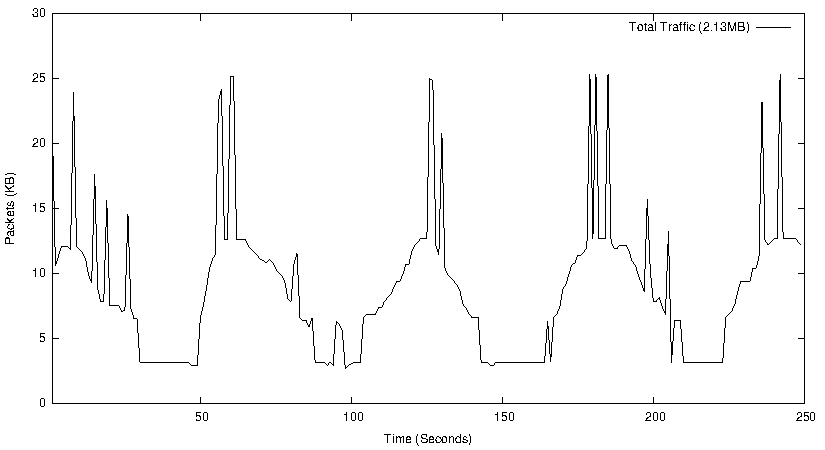
\includegraphics[scale=1.0]{indi10packet-distribution.pdf}
\caption{A histogram plotting the amount of network traffic INDI propagates onto the network per second for Poisson-10.} 
\label{indi:fig:indi-10-traffic}
\end{figure}

The ``success rate'' results for the various levels of $SDD_{a}$ and $SDD_{d}$ values for the complete set of experiments is provided in table \ref{table:jmdns:comparison}.  It is clear that INDI out-performs JmDNS across the board, reaching 100\% for $SDD_{a}$ values of 2 seconds and above and $SDD_{d}$ values of 5 seconds or above.   In fact, an $SDD_{a}$ value of 1.8 and  an $SDD_{d}$ value of 2.7 is enough to achieve 100\% in all test cases for INDI covered in this study, the average being significantly less. This is discussed in depth in Section \ref{indi:sec:indepth}.  
 
\begin{figure}
\centering
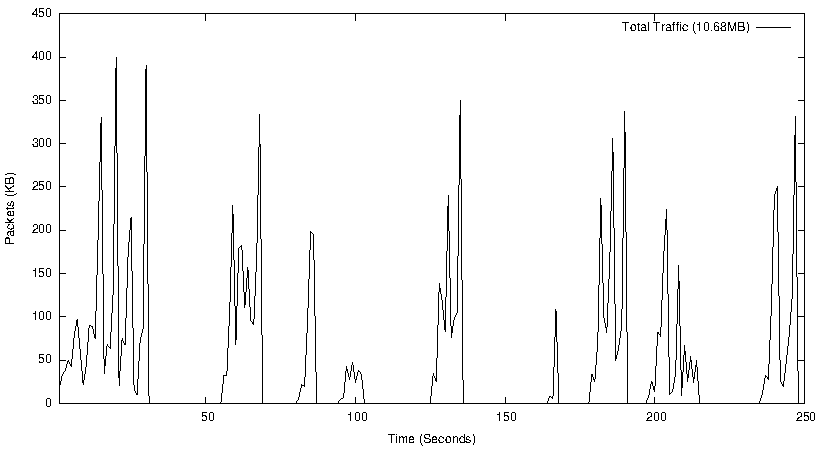
\includegraphics[scale=1.0]{jmdns10packet-distribution.pdf}
\caption{A JmDNS traffic histogram showing the Poisson-10 case.   } 
\label{indi:fig:jmdns-10-traffic}
\end{figure}
 

JmDNS on the other hand due of its design cannot meet the requested QoS limits.  The dynamics of the network and services is far too extreme for the conservative mDNS timer settings, designed solely for use on a LAN. Also, the extra redundancy in the messaging involved in an mDNS handshake, increases the latency too much to meet the required QoS. This is discussed in more detail in the next section to cohabit with the mDNS handshaking discussion and bandwidth requirements.   The more general issues of responsiveness are discussed in Section \ref{indi:sec:indepth}.

\subsection{Overhead Analysis}   
\label{subsec:overhead}

\begin{figure}
\centering
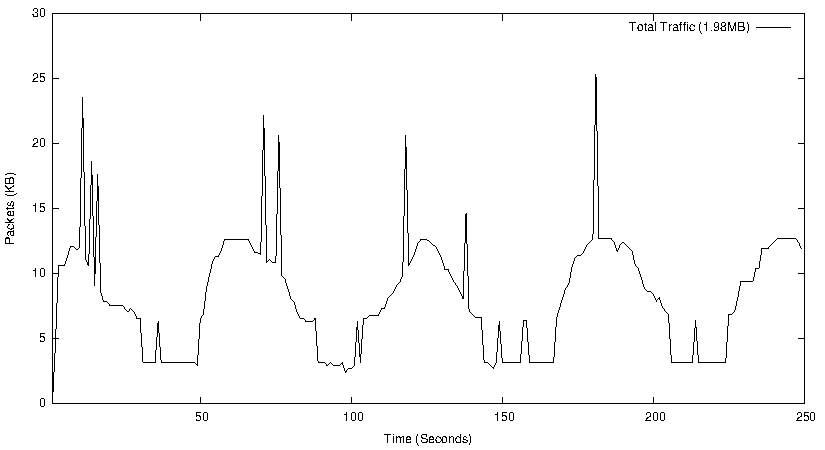
\includegraphics[scale=1.0]{indi20packet-distribution.pdf}
\caption{An INDI traffic histogram showing the Poisson-20 case.} 
\label{indi:fig:indi-20-traffic}
\end{figure}

At a high level, INDI and JmDNS operate in different modes.  INDI employs more of a proactive approach when addressing mobility whereas JmDNS has a defined sequence of message handshakes between JmDNS responders, which follow a combination of proactive and reactive solicitation.  However, in the JmDNS case, this interaction has a high short-term burst rate of several seconds and then a period of inactivity in transmitting messages across the network.  For INDI however, it proactively announces at a specific interval (1 second in these emulations) through the entire emulation. Therefore, although there are some minor peaks during service advertisement switch over in the INDI overhead histogram, this explains why is it is far more smooth overall.   Figures \ref{indi:fig:indi-10-traffic}, \ref{indi:fig:jmdns-10-traffic}, \ref{indi:fig:indi-20-traffic}, \ref{indi:fig:jmdns-20-traffic}, \ref{indi:fig:indi-30-traffic} and \ref{indi:fig:jmdns-30-traffic} show the traffic overhead caused by INDI and JmDNS for the three test cases covering Poisson mean intervals of 10, 20 and 30 seconds, respectively.

\begin{figure}
\centering
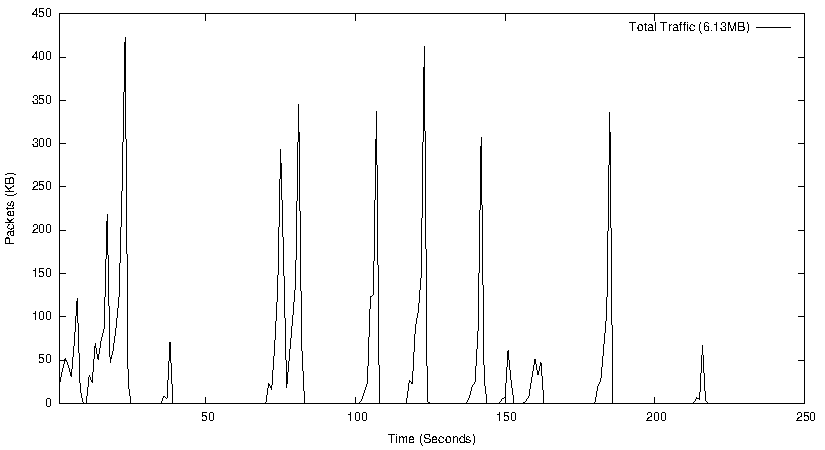
\includegraphics[scale=1.0]{jmdns20packet-distribution.pdf}
\caption{A JmDNS traffic histogram showing the Poisson-20 case.   } 
\label{indi:fig:jmdns-20-traffic}
\end{figure}

 Figures \ref{indi:fig:indi-10-traffic} and \ref{indi:fig:jmdns-10-traffic} show the traffic for the 10  second Poisson interval case.   It might seem clear from the proactive scheme that INDI sends out far more service advertisement requests with a shorter interval, creating consistent periodic traffic throughout the duration of the emulation. However, INDI messages are sent once and are not subjected to a number of handshakes with the client. In these experiments therefore, we can see that there are a lot less INDI messages and far less bandwidth consumed overall.  For each service advertisement request, JmDNS exchanges tens of message every time a service arrives onto the network and then remains quiet until the next advert comes onto the network.  This results in a far higher traffic burst rate and an accumulation of messages. Looking more closely at the scales in Figures \ref{indi:fig:indi-10-traffic} and \ref{indi:fig:jmdns-10-traffic}, we can in fact see that the JmDNS scale is one order of magnitude higher than that of INDI and hence, the total traffic consumed for INDI is 2.13 MB for the duration of the experiment, compared to 10.68MB for JmDNS. 
  
\begin{figure}[htb]
\centering
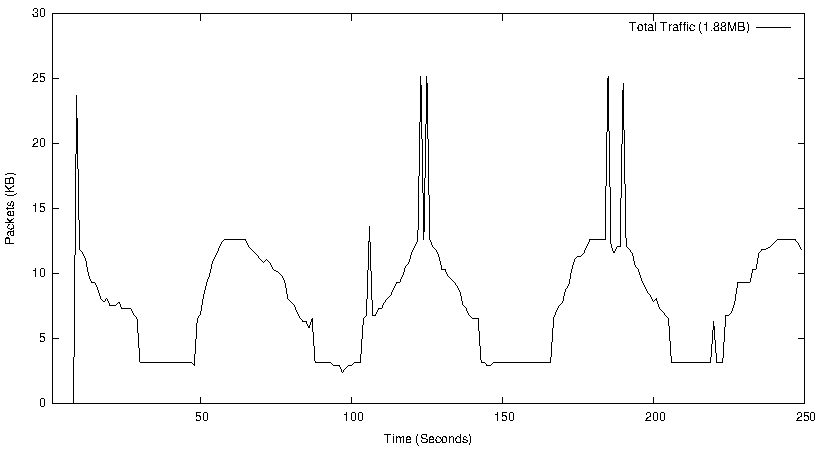
\includegraphics[scale=1.0]{indi30packet-distribution.pdf}
\caption{An INDI traffic histogram showing the Poisson-30 case.   } 
\label{indi:fig:indi-30-traffic}
\end{figure}

% change all to Poisson-10

 Considering the rather significant gains in success rates for INDI compared to JmDNS, it is somewhat surprising at first glance that JmDNS generates more traffic.  However, let's consider further evidence from our previous experiments \cite{Macker2011}.  In this experiment, we used Wireshark\footnote{http://www.wireshark.org/}, a sophisticated tool for capturing and parsing packets on the network, to observe the messages exchanged for a single service advertisement from INDI in Proactive mode and JmDNS, using a simple loopback network connector.  It was found that upon bootstrapping and discovering the first service on the network, a JmDNS node traverses through various stages e.g. server probing (three times), announcing (three two times) for resolving addresses and thereafter a further sequence for resolving services e.g. probers, announcers, and then type, service and service info resolvers.   This verbose activity results in 25 messages being exchanged between two JmDNS services to make the first discovery.  Thereafter, only the service sequence is followed but again this is several exchanges per service advertisement and thus causes large peaks at service interval times.  
 
The explanation for this extra bandwidth has already been discussed in Section \ref{sec:background}.  Since mDNS was designed to cover all LAN use cases, this is bound to have a knock on effect in terms of redundancy. Although a factor of 5 might at first glance seem high, mDNS attempts to deal with all combinations of clients and servers arriving at different times and is designed for an environment where services do not come onto the network very frequently.  Therefore, for example, over the course of several hours with one service arriving per hour (which is more in tune with the design requirements of mDNS), mDNS would indeed perform more efficiently than INDI set in proactive mode.  And although INDI could in theory be tuned to exhibit a similar behavior to mDNS by using a combination of proactive and reactive modes, it would unlikely to provide any benefit at all for use within a LAN.    So, the choice between the two for bandwidth efficiency depends completely on the dynamic nature of the services and the environment they are run in. Within a MANET however, the gains are clearly in the favor of INDI.   

\begin{figure}[htb]
\centering
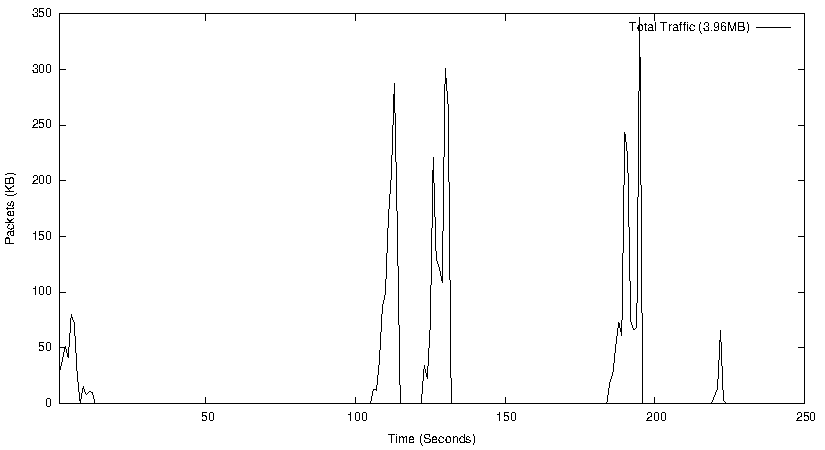
\includegraphics[scale=1.0]{jmdns30packet-distribution.pdf}
\caption{A JmDNS traffic histogram showing the Poisson-30 case.   } 
\label{indi:fig:jmdns-30-traffic}
\end{figure}

Figures \ref{indi:fig:indi-20-traffic}, \ref{indi:fig:jmdns-20-traffic}, \ref{indi:fig:indi-30-traffic} and \ref{indi:fig:jmdns-30-traffic} for Poisson-20 and Poisson-30 cases tell a similar story.  However, the results are not so extreme because there are less adverts being advertised during the course of the emulation.  For the 20 second interval, there are 15 service advertisements and for the 30 second interval, there are only 7. Therefore, the amount of traffic consumed is less for all cases.  The reductions in traffic for JmDNS are significant and depend directly on the number of advertisements. For example, whereas the JmDNS traffic for Poisson-10 was  10.68MB, Poisson-20 was 6.13 and Poisson-30 was 3.96, for INDI the traffic rates were 2.13, 1.98 and 1.88 MBs, respectively.  Even with 7 advertisements across the 250 second duration (less than two per minute), INDI still consumed less than half the traffic of JmDNS.  Further, as the result in table \ref{table:jmdns:comparison} shows, the success rates for INDI are more than twice that of JmDNS in these cases. For traffic therefore, there is little evidence from this study that the extra bandwidth consumed by JmDNS is having any effect of service discovery in this environment.  In the next section, we look at the the Poisson-10  and study the advert distribution and the reasons for the success differences between INDI and JmDNS more closely.


\subsection{A Closer Look at 10 Second Interval Case}   
\label{indi:sec:indepth}

\begin{figure}[htb]
\centering
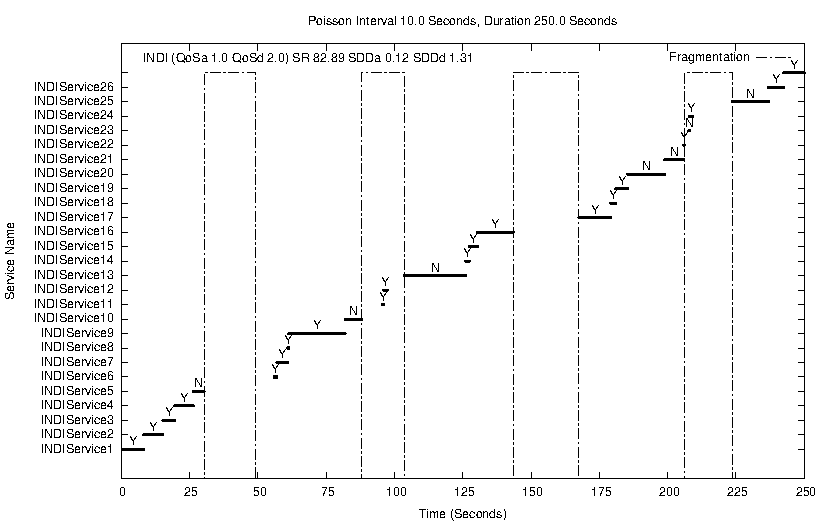
\includegraphics[scale=1.0]{indi10-1-2-results-distribution.pdf}
\caption{INDI: Shows the fragmentation pattern that affects the services' availability, the arrival and departure of each advert and the corresponding indication of successful detection of that advert (Y = success, N = failure).} 
\label{indi:fig:poisson-10-1-2}
\end{figure}

By observing the location and duration of the adverts during the course of the emulation for the Poisson-10 case, we discuss in this Section why certain adverts succeeded to be detected by a discovery systems and why others failed. Although we have 32 different cases in this category, we consider the two extreme cases here for illustration:

\begin{enumerate}
\item An  $SDD_{a}$ of 1 second and an $SDD_{d}$ 2 seconds.
\item An $SDD_{a}$ of 10 seconds and an $SDD_{d}$ of 20  seconds.
\end{enumerate}

In Figure \ref{indi:fig:poisson-10-1-2}, we show the performance of INDI when it has been requested to meet an $SDD_{a}$ of 1 second and an $SDD_{d}$ of 2 seconds. This plot shows a number of different things.   First, it overlays the connectivity diagram that representations the fragmentation in the network shown  in Figure \ref{indi:fig:emulationconnectivity}.  It then shows each service advertised during the course of the emulation (as per Figure \ref{indi:fig:poisson-10-adverts}) labelled by name on the y axis and annotated by a Y (success) or N (failure) if the service discovery system was able to detect that advert or not.   The services are also calibrated to show their visibility for consumers 5-9 after the fragmentation has been applied (as per Figure \ref{indi:fig:poisson-10-adverts-frag}). Finally, the statistics are provided about this run as a label at the top part of the graph, in the form:

\begin{verbatim}
INDI (QoSa 1.0 QoSd 2.0) SR 82.89 SDDa 0.12 SDDd 1.31
\end{verbatim}


\noindent which describe the parameters defined in Section \ref{sec:methodology}. This example shows that the INDI discovery system when applied to QoS parameters of $SDD_{a}$ of 1 second and $SDD_{d}$ of 2 seconds achieve as success rate (SR) of 82.89\%, an average service detection delay for arrival of 0.12 seconds and an average service detection delay for departure of 1.31 seconds.   

\begin{figure}[htb]
\centering
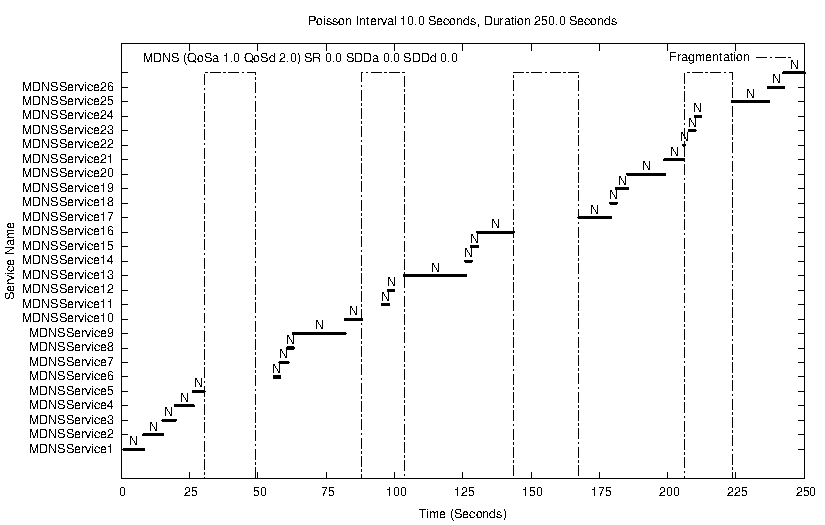
\includegraphics[scale=1.0]{jmdns10-1-2-results-distribution.pdf}
\caption{JmDNS: Successful service detection (Y = success, N = failure).} 
\label{jmdns:fig:poisson-10-1-2}
\end{figure}

Although INDI succeeds in detecting all of the services in the emulation, it cannot meet this QoS rate to the full. Looking in more detail at Figure \ref{indi:fig:poisson-10-1-2}, we can see that services around the fragmentations cause the most issues and since a success rate is applied to all consumers for each service, then the fragmented consumers are having a larger impact here.   The explanation for this affect is to do with the quantization of the proactive readvertisement interval and its alignment to services appearing and disappearing from the network.  Since INDI employed a proactive service announcement scheme (of rate 1 per second and a TTL of 2 seconds) for this experiment, these results are somewhat expected.   And upon further finer-grained analysis of the data, it was found in fact that an $SDD_{a}$ value of 1.8 and  an $SDD_{d}$ value of 2.7 is enough to achieve 100\% in all test cases for INDI covered in this study.  

The $SDD_{d}$ rate can be explained because when a service is deleted there is a slightly delay (100-200 ms) on the server whilst it starts the \emph{RecordReaper}  to detect the advert is expired.  During this time, it is possible in some case for the producer to proactively readvertise the service for a further TTL of 2 seconds.  And then on the service side,  since it takes 300-400 milliseconds to register a service in some cases, the range of 2.7 seconds can be expected in extreme circumstances.   

To combat these affects, INDI allows the tuning of both the proactive service announcement interval and the TTL for a service advertisement. Decreasing these values can improve responsiveness of the system, with the overhead of increased network bandwidth.  The decision for setting these values is application and network dependent. 

\begin{figure}[htb]
\centering
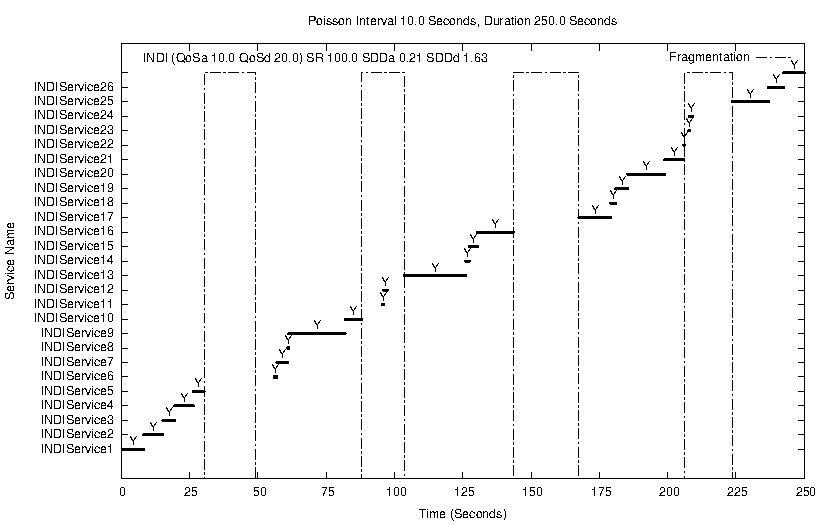
\includegraphics[scale=1.0]{indi10-10-20-results-distribution.pdf}
\caption{INDI: Successful service detection (Y = success, N = failure).} 
\label{indi:fig:poisson-10-10-20}
\end{figure}


In Figure \ref{jmdns:fig:poisson-10-1-2}, the story is quite different.  JmDNS was unable to discover any services using these values for the QoS metric. Not only does JmDNS suffer from a finite advertisement sequence (several seconds normally) and therefore misses a number of adverts that go out of range because of this, it also does not provide sufficient timely notification internally when success has been reached. Therefore, JmDNS needs far more time to respond successfully to service advertisements and therefore, it cannot meet the dynamics exhibited here and the level of QoS defined.  

This is explained again by the significantly different design priorities for mDNS when discovering services.  Rather than dealing with responsiveness, it performs multiple queries in order to ensure the discovery of the new longer lived services but also, it attempts to deal with maintaining the state of node IP addresses in case of conflicts.  This extra level of state maintenance creates an extra overhead on the network that introduces more traffic and a longer delay in the initial discovery. This is therefore not a failing of JmDNS but rather a mismatch of its intended purpose. However, it does stress the importance on the level of configurability for offering flexible modes and timers that INDI strives to achieve.

\begin{figure}[htb]
\centering
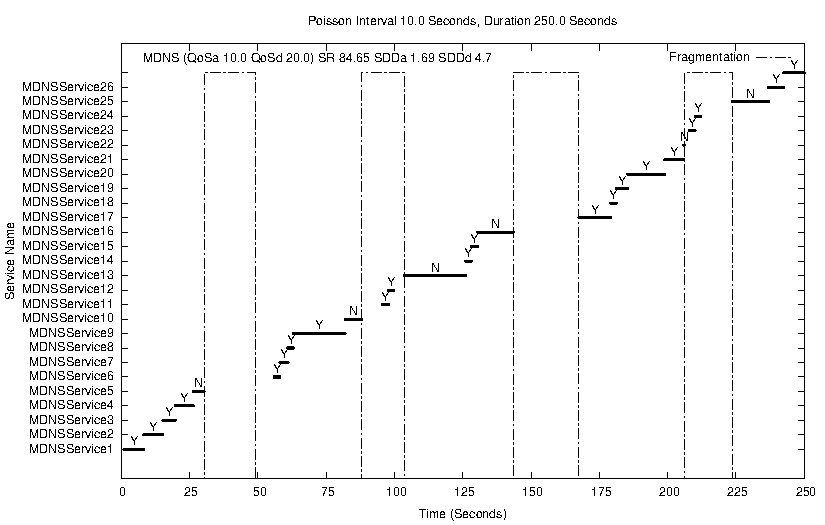
\includegraphics[scale=1.0]{jmdns10-10-20-results-distribution.pdf}
\caption{JmDNS: Successful service detection (Y = success, N = failure).} 
\label{jmdns:fig:poisson-10-10-20}
\end{figure}

The extended time period for $SDD_{a}$ of 10 seconds and $SDD_{d}$ of 20 seconds in Figure \ref{indi:fig:poisson-10-10-20} provides plenty of headroom for INDI to meet the expectations stated in the QoS. INDI achieves 100\% success with a delay of 0.21 seconds for the discovery of a service and an average of 1.63 seconds for the detection of a service when it departs from the network.

In Figure \ref{jmdns:fig:poisson-10-10-20} however, with a $SDD_{a}$ of 10 second and $SDD_{d}$ of 20 seconds, JmDNS  cannot achieve 100\%.  Its success rate is 84.65\% and it has a delay of 1.69 seconds for the discovery of a service (1.48 more than INDI) and an average of 4.7 seconds for the detection of a service (3.07 seconds more than INDI) when it departs from the network.

It is clear here, even with generous QoS constraints, that JmDNS suffers from the fragmentation of Consumers 5 to 9 when discovering services. It failed on \emph{MDNSService} services numbered 5, 10, 13, 16, 21 and 24.  All of these services either joined or left the network during the advertisement.  This can be explained by the follow reasons:

\begin{itemize}
\item \textbf{Services disappearing through fragmentation:} When a service is fragmented, mDNS has no mechanism for detecting this event. The TTL for an mDNS advert is 2 hours by default and since the producer does not know that consumers have gone out of range, it cannot notify them, and even if it did, there would be no connection.   Therefore, mDNS will always fail in this respect.  For INDI, it implements an adjustable TTL, which determines the rate at which adverts need to be refreshed and therefore it can detect absences.

\item \textbf{Services reappearing after fragmentation:} When a service reappears after a fragmentation, then mDNS can only discover it if it appears within its finite sequence of handshakes when a new service is advertised.  Therefore, MDNSService 17 was discovered by mDNS because it was advertised only a second or so before it came back into range and therefore within the normal mDNS handshaking sequence range.  Other advertisements could not be discovered because the interval was beyond its probing and announcement phases. 
\end{itemize}
 
